\documentclass[]{article}
\usepackage[utf8]{inputenc}
\usepackage{polski}
\usepackage{graphicx}
\graphicspath{ {./images/} }
\usepackage[margin=0.5in]{geometry}
\usepackage{gensymb}
\usepackage{textcomp}
\usepackage{siunitx}
\usepackage{float}

\begin{document}

\begin{figure}[tp!]
	\center{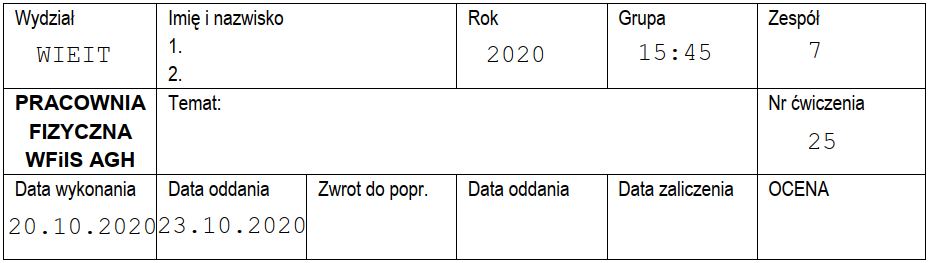
\includegraphics{F}}
\end{figure}

\begin{center}
	\section*{Interferencja fal akustycznych }
	\emph{Dzmitry Mikialevich}
\end{center}
\begin{center}
	\emph{Wojciech Sikora}
\end{center}
\tableofcontents
\newpage

\section{Wstęp}

\subsection{Cel ćwiczenia}
Pomiar prędkości dźwięku w powietrzu przy użyciu rury Quinckego. Wyznaczenie wykładnika \(\kappa\) w
równaniu adiabaty.

    
\subsection{Opis ćwiczenia}
Doświadczenie wykonujemy z wykorzystaniem równania fali dzwiękowej: \[y=y_msin(kx-\omega t)\]
\newline
Superpozycja dwóch fal jest określona przy pomocy równania:
\[y=y_msin(\omega t-\phi)\] gdzie: \[y_m=\sqrt{y^2_m_1+y^2_m_2+2y_m_1y_m_2cosk(x_1-x_2) }\]
\newline
Celem było obliczenie odległości pomiędzy kolejnymi minimami amplitudy nakładających się
dwóch fal. W ten sposób otrzymaliśmy długość fali, która pozwoliła nam obliczyć prędkość dźwięku
ze wzoru:
\[\upsilon = f \cdot \lambda\]
\newline
Na dokładność wykonanego pomiaru wpływają czynniki takie jak temperatura powietrza, czy -
w mniejszym stopniu - jego wilgotność.
    
\section{Układ Pomiarowy}
W skład układu pomiarowego weszły następujące elementy:
\newline

1. Rura Quinckego


2. Generator mocy 20 Hz – 20 kHz


3. Licznik do odczytu częstotliwości


4. Oscyloskop 

\begin{figure}[h]
	\center{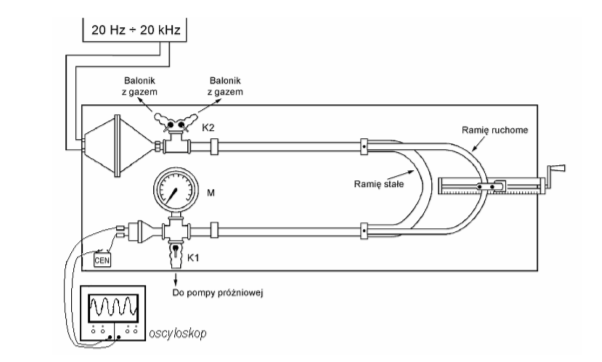
\includegraphics{A_1}}
	\textbf{\caption{Badany układ rury Quinckego}}
	
\end{figure}





\section{Przebiegi doświadczenia}
W ramach doświadczenia przeprowadziliśmy 11 serii pomiarów odległości między minimami amplitudy przy różnych częstotliwościach dźwięku. Z każdej serii pomiaru uzyskaliśmy średnią, która pozwoliła ustalić długość fali, a w konsekwencji - prędkość rozchodzenia się dźwięku. Badane częstotliwości były z zakresów 800-1200 Hz oraz 2000-3200 Hz

\section{Wyniki Pomiarów}


	\begin{table}[h]
		\centering
		\begin{tabular}{|l|l|l|l|l|l|l|l|l|l|l|l|l|}
			\hline
Częstotliwość f& \multicolumn{5}{|c|}{\begin{tabular}{@{}c@{}}Położenia \\ Kolejnych minimów [mm]\end{tabular}} & \multicolumn{4}{|c|}{ \begin{tabular}{@{}c@{}}Różnica położeń \\ Kolejnych minimów [mm]\end{tabular}} & Średnia różnica & Długość fali &  \begin{tabular}{@{}c@{}}Prędkość\\Dzwięku\end{tabular} \\ \hline

  [Hz] & \(a_1\) & \(a_2\) & \(a_3\) & \(a_4\) & \(a_5\) & \(\Delta_1\) & \(\Delta_2\) & \(\Delta_3\) & \(\Delta_4\) & [mm] & [mm] & [m/s]  \\ \hline
873 & 133 & 263 &  &  &  & 130 &  &  &  & 130 & 260 & 226,98 \\ \hline
936 & 59 & 255 & 438 &  &  & 196 & 183 &  &  & 189,5 & 379 & 354,744 \\ \hline
997 & 65 & 168 & 245 & 418 &  & 103 & 77 & 173 &  & 117,66 & 235,32 & 234,614 \\ \hline
1136 & 85 & 218 & 370 &  &  & 133 & 152 &  &  & 142,5 & 285 & 323,76 \\ \hline
2002 & 71 & 154 & 247 & 335 & 421 & 83 & 93 & 88 & 86 & 87,5 & 175 & 350,35 \\ \hline
2128 & 58 & 135 & 219 & 301 & 380 & 77 & 84 & 82 & 79 & 80,5 & 161 & 342,608 \\ \hline
2238 & 45 & 124 & 200 & 276 & 355 & 79 & 76 & 76 & 79 & 77,5 & 155 & 346,89 \\ \hline
2368 & 11 & 41 & 120 & 152 & 223 & 30 & 79 & 32 & 71 & 53 & 106 & 251,008 \\ \hline
2555 & 40 & 76 & 150 & 214 & 286 & 36 & 74 & 64 & 72 & 61,5 & 123 & 314,265 \\ \hline
2796 & 34 & 98 & 158 & 220 & 280 & 64 & 60 & 62 & 60 & 61,5 & 123 & 343,908 \\ \hline
3027 & 31 & 86 & 147 & 203 & 261 & 55 & 61 & 56 & 58 & 57,5 & 115 & 348,105 \\ \hline

			
		\end{tabular}
		\textbf{\caption{Pomiary położeń minimów i obliczenia prędkości dzwięku }
		}
	\end{table}
\newline
\textbf{Temperatura w pomieszczeniu: }\(T = \SI{21,5}{\celsius}= 294,65\:K\),
\textbf{Niepewność pomiarowa} \(u(T) =\SI{0,5}{\celsius} = 0,5\:K\)

\section{Opracowanie wyników Pomiarów}
    \subsection{Obliczenia i niepewności}
    \subsubsection{Obliczenia}
Za pomocą następujących wzorów uzyskaliśmy wartośći:\newline \newline
Różnic położeń kolejnych minimów: \[\Delta_i = a_{i+1} - a_i\]
Średnią róźnicę:  \[\overline{\Delta} = \frac{\sum \Delta_i}{n}\]
Długość fali: \[\lambda = 2 \cdot \overline{\Delta}\]
Prędkość fali: \[\upsilon = f \cdot \lambda\]
Gdzie:\newline \(a_i\) - i-ty minimum,\newline
n - ilość różnic położeń kolejnych pomiarów, \newline
f - częstotliwość. \newline
    \subsubsection{Niepewności}
	\begin{table}[H]
		\centering
		\begin{tabular}{|l|l|l|l|l|}
			\hline
Częstotliwość f [Hz] & Średnia różnica [mm]& \(u(\overline{\Delta})\) [mm] & Prędkość dzwięku \([m/s^2]\)& \(u(\upsilon)\)  \([m/s^2]\)\\ \hline
873 & 130 & 2 & 226,98 & 1,75 \\ \hline
936 & 189,5 & 6,5 & 354,744 & 6,09 \\ \hline
997 & 117,66 & 28,67 & 234,614 & 28,59 \\ \hline
1136 & 142,5 & 9,5 & 323,76 & 10,8 \\ \hline
2002 & 87,5 & 2,1 & 350,35 & 4,2 \\ \hline
2128 & 80,5 & 1,56 & 342,608 & 3,32 \\ \hline
2238 & 77,5 & 0,87 & 346,89 & 1,95 \\ \hline
2368 & 53 & 12,82 & 251,008 & 30,36 \\ \hline
2555 & 61,5 & 8,78 & 314,265 & 22,44 \\ \hline
2796 & 61,5 & 0,96 & 343,908 & 2,69 \\ \hline
3027 & 57,5 & 1,33 & 348,105 & 4,03 \\ \hline
		\end{tabular}
		\textbf{\caption{Niepewności typu A }
		}
	\end{table}
    Na Tablicy 2 przedstawione są niepewności pomiaru typu A, oprócz niepewności dla f = 873 Hz, która była oszacowana jako 2 mm.
    
    
    
    
    \subsection{Wykres otrzymanych wartości \mathbf{v} w funkcji  częstotliwości drgań źródła \mathbf{f}}
    
\begin{figure}[H]
	\center{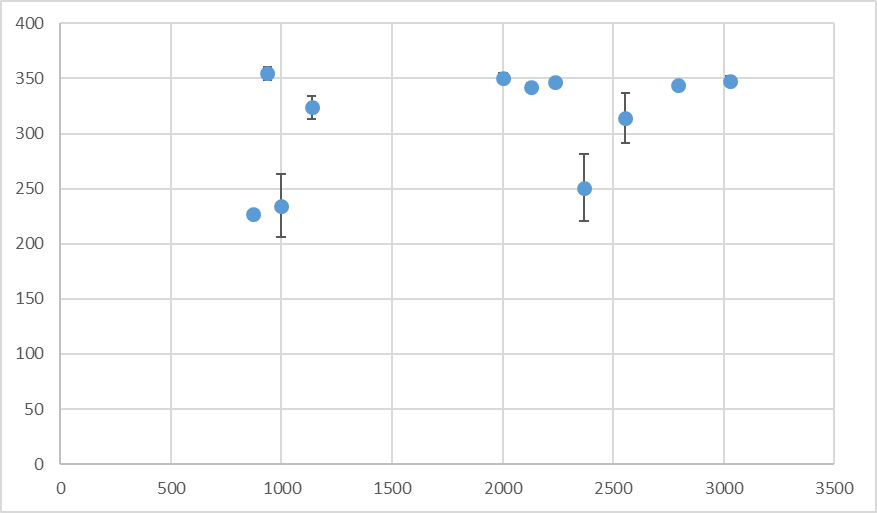
\includegraphics{Graphic}}
	\textbf{\caption{Wykres otrzymanych wartości \mathbf{v} w funkcji  częstotliwości drgań źródła \mathbf{f}}}
\end{figure}
    \subsection{Wartość średnia  \mathbf { \(\bar v\)} i niepewność standardową \mathbf {u(v)}}
    Jak widać z Rysunku 2 i Tablicy 2 mamy kilka błędów grubych, np. dla częstotliwości 997, 2368 i 2555 Hz, \(u(\upsilon)\) dużo przekracza oczekiwaną wartość. W związku z tym pomjamy te częstotliwości w dalszych obliczeniach.\newline \newline
Wartość średnia prędkości: 
\[ \overline \upsilon = \frac{\sum \upsilon_i}{n} = 329,67\: m/s\]
Niepewność standartowa: 
\[u(\upsilon) = \sqrt{\frac{\sum({x_i - \overline x})^2}{n(n-1)}} = 15,02\:m/s\]
Taka duża wartość niepewności jest związana z trudnością wyznaczania dokładnego miejsca minimum i niedokładne mierzenie średniej odległości między kolejnymi odchyleniami. 

\newpage

\subsection{Prędkość dzwięku dla temperatury \(t_0=0\:\celsius\)}

Korzystając ze wzoru na prędkość dźwięku w gazach przeliczamy zmierzoną prędkość na prędkość \newline dla temperatury \(T_0 = 0\:\celsius = 273.15\:K\)
\newline
Zmierzona przed rozpoczęciem pomiarów temperatura pomieszczenia wynosiła \(T=21.5\:\celsius=294.65\:K\)

\[\upsilon_0=\overline\upsilon\sqrt{\frac{T_0}{T}}\]
\[\upsilon_0=317,41\:m/s\]

\subsection{Porównanie obliczonej prędkości dźwięku z wartością tablicową}
Korzystając z prawa przenoszenia niepewności:
\[u(\upsilon_0)=u(\upsilon)\sqrt{\frac{T_0}{T}}=13,92\:m/s\]
Przyjmując współczynnik k = 2 liczymy niepewność rozszerzoną:
\[U(\upsilon_0)=k \cdot u(\upsilon_0)=2 \cdot 13,92=27,84\:m/s\]
Wartość tablicowa prędkości dźwięku dla suchego powietrza w temperaturze 0\celsius\vspace{} wynosi 331,5 m/s.
\[|331,5-317,41|=14,09<27,84=U(\upsilon_0)\]
\newline
Wartość tablicowa jest mniejsza od otrzymanych wyników pomiarów, a obliczona niepewność większa niż faktyczny błąd.


\subsection{Wartość wykładnika adiabaty}
Korzystając ze wzoru na prędkość dźwięku w gazach:
\[\upsilon=\sqrt{\frac{\kappa RT}{\mu}}\]
Gdzie \(T\) - temperatura bezwzględna, \(R\) - stała gazowa, \(\mu\) - masa molowa molekułu gazu, a \(\kappa\) - wykładnik adiabaty.\newline \newline


Obliczamy masę molową dla powietrza (mieszaniny azotu (78\%), tlenu (21\%) i argonu(1\%)) jako
średnią ważoną mas molowych składników:

\[\mu=0,78 \cdot 28 + 0,21 \cdot 32 + 0,01 \cdot 40 = 29,86\:\frac{g}{mol} = 0,02986\:\frac{kg}{mol}\]
Stała \(R=8,31\:\frac{J}{mol\cdot K}\) \newline \newline

Przekształcamy wzór, uzyskując wykładnik adiabaty:
\[\kappa=\frac{\mu \upsilon^2}{RT}=1,28\] \newline
Z prawa przenoszenia niepewności względnej:
\[u(\kappa)=\sqrt{[\frac{2\upsilon \mu}{RT}u(\upsilon)]^2+[\frac{v^2\mu}{RT^2}u(T)]^2}=0,87\]
\newpage
\subsection{Wnioski}
\begin{itemize}
		\item Dowiedzieliśmy się, że za pomocą rury Quinckiego jest możliwe szacowanie prędkości dzwięku w dowolnym gazie.
		\item  Obliczono średnią prędkość dzwięku \(\upsilon = 329,67\: m/s\) z niepewnością \(u(\upsilon) =15,02 \: m/s\) w temperaturze T = 294,65 [K] zmierzonej z niepewnością u(T) = 0,5 K. W związku z niedokładnym oszacowaniem minimumów w niektórych przypadkach (szczególnie dla małych częstotliwości) wartość niepewności jest duża, co nie przeszkadza w analizie doświadczenia i uzyskania prędkości średniej dzwięku, która mieści się w niepewności pomiarowej, i dalszym szacowaniu wartości adiabaty.
		\item Z wykorzystaniem pomiarów obliczono prędkość dźwięku w temperaturze równej T=273,15 K, która wyniosła  \(\upsilon_0=317,41\: m/s\) z niepewnością rozszerzoną równą \(u(\upsilon_0)=27,84\:m/s\)
		\item Obliczono wykładnik adiabaty \(\kappa = 1,28\) z niepewnością \(u(\kappa)=0,87\) co zgadza się wartością tablicową
	\end{itemize}
\end{document}